\section{Theoretical Background}
% \addcontentsline{toc}{section}{Theoretical Background}
\fancyhead[R]{Theoretical Background}

\subsection{Principles of Enzymology}
\label{sec:Principles of Enzymology}

Enzymology is the scientific study of enzymes, which are biological catalysts that accelerate biochemical reactions in living organisms. Enzymes are crucial for various cellular processes, including metabolism, DNA replication, and signal transduction. They are highly specific, meaning each enzyme typically catalyzes only one type of reaction or interacts with a specific substrate. This specificity arises from the enzyme’s unique three-dimensional structure, which includes an active site where the substrate binds and the reaction occurs.
\autocite{robinsonEnzymesPrinciplesBiotechnological2015}

Enzymes are classified based on the types of reactions they catalyze, according to a system established by the Enzyme Commission (EC). This classification groups enzymes into six main classes: Oxidoreductases, Transferases, Hydrolases, Lyases, Isomerases, and Ligases. For example, Oxidoreductases catalyze oxidation-reduction reactions, where the transfer of electrons occurs between molecules. Understanding these classifications helps in predicting the enzyme’s role in biochemical processes. Digestive enzymes like amylase break down starch into sugars, facilitating digestion. Similarly, enzymes in laundry detergents help break down protein stains, making them easier to remove. The specificity of enzymes for their substrates is a key feature that enables them to perform their roles in various biochemical pathways with high precision. The following figure gives a brief overview of the seven classes of enzymes according to the EC classification system:

\begin{compactenum}
    \item \textbf{Oxidoreductases:} These enzymes catalyze oxidation-reduction reactions, where the transfer of electrons occurs between molecules.
    \item \textbf{Transferases:} These enzymes transfer functional groups from one molecule to another.
    \item \textbf{Hydrolases:} These enzymes catalyze the hydrolysis of various bonds, including ester, glycosidic, peptide, and others.
    \item \textbf{Lyases:} These enzymes add or remove groups to form double bonds, without hydrolysis or oxidation.
    \item \textbf{Isomerases:} These enzymes catalyze the rearrangement of atoms within a molecule, leading to isomerization.
    \item \textbf{Ligases:} These enzymes catalyze the joining of two molecules with the simultaneous hydrolysis of a diphosphate bond in ATP or a similar triphosphate.
    \item 
\end{compactenum}

For example, the enzyme tripeptide aminopeptidase has the EC number "3.4.11.4", where the first digit (3) represents the class (Hydrolases in this case), the second digit (4) represents the subclass (hydrolases that act on peptide bonds), the third digit (11) represents the sub-subclass (Hydrolases that cleave off the amino-terminal amino acid from a polypeptide), and the fourth digit (4) represents the serial number of the enzyme within the sub-subclass (Hydrolases that cleave off the amino-terminal end from a tripeptide). This systematic classification allows researchers to identify enzymes based on their catalytic activities and biochemical properties. \autocite{EnzymeNomenclatureRecommendations1994}

The distribution of EC numbers across the six classes is not uniform, with hydrolases being the most abundant class, reflecting the importance of hydrolysis in biological processes. The following figure shows the distribuion of EC numbers across all four levels of the classification system:

\begin{table}[hbt]
    \centering
    \begin{tabular}{@{}ll@{}}
    \toprule
    \textbf{EC Level} & \textbf{Number of classes} \\ \midrule
    1                 & 7                          \\
    2                 & 79                         \\
    3                 & 320                        \\
    4                 & 7876                       \\ \bottomrule
    \end{tabular}
    \caption{Distribution of EC numbers across different levels of the classification system.}
    \label{tab:ec-level-distribution}
\end{table}

The table shows an unbalanced distribution of EC numbers across the four levels of the classification system, with a higher number of classes at the lower levels. This distribution reflects the increasing specificity and diversity of enzyme functions as it moves from higher to lower levels of the classification system. The high number of classes at the fourth level highlights the complexity of enzyme functions and the challenges associated with predicting enzyme classes accurately. This complexity will be further discussed in the subsequent sections.

Enzymes are not only classified based on their catalytic activities but also based on their biological functions. The three-dimensional (3D) structure of enzymes is fundamental to their function. Enzymes are composed of one or more polypeptide chains that fold into specific shapes to form the active site. The active site is where substrate molecules bind and undergo a chemical reaction. The enzyme structure serves as a scaffold to support and correctly position the active site for optimal catalytic activity.

\begin{figure}[hbt]
    \centering
    \begin{minipage}[t]{\textwidth}
    \caption{Organisation of enzyme structure and lysozyme example.}
    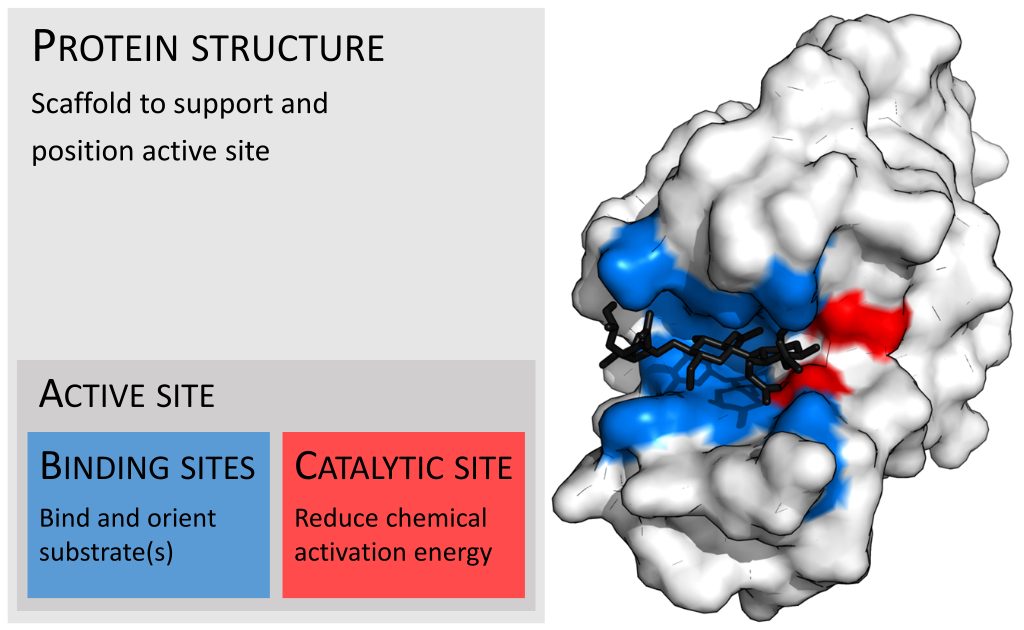
\includegraphics[width=.7\textwidth]{img/EnzymeStructure.svg.png}\\
    \source{\autocite{shafeeEnglishOrganisationEnzyme2015}}
    \label{fig:EnzymeStructure}
    \end{minipage}
\end{figure}

The overall structure of the enzyme provides the framework that supports and positions the active site. This structure is critical for the enzyme's stability and functionality. The enzyme's polypeptide chains fold into a unique 3D shape, creating a specific environment for the active site.
The active site includes two critical regions: binding sites and the catalytic site. The binding sites (highlighted in blue) are regions where substrates bind to the enzyme. These sites ensure that the substrates are properly oriented for the reaction. The catalytic site (highlighted in red) is the region where the chemical reaction occurs. The catalytic site often contains amino acids with specific functional groups that participate directly in the reaction, reducing the activation energy required for the reaction to proceed.

The Key-Lock Principle, first proposed by Emil Fischer in 1894, is a model for understanding the specificity of enzyme-substrate interactions. According to this principle, the enzyme (lock) has a specific active site shape that only fits a particular substrate (key). This model emphasizes the specificity of enzyme-substrate interactions and how enzymes are highly selective for their substrates. This principle is fundamental to understanding enzyme function and the mechanisms of catalysis. The specificity of these interactions is crucial for predicting enzyme activities because it determines the substrates that can bind to the enzyme and undergo catalysis.

\begin{figure}[hbt]
    \centering
    \begin{minipage}[t]{\textwidth}
    \caption{Lock-and-key model that explains the selectivity of enzymes}
    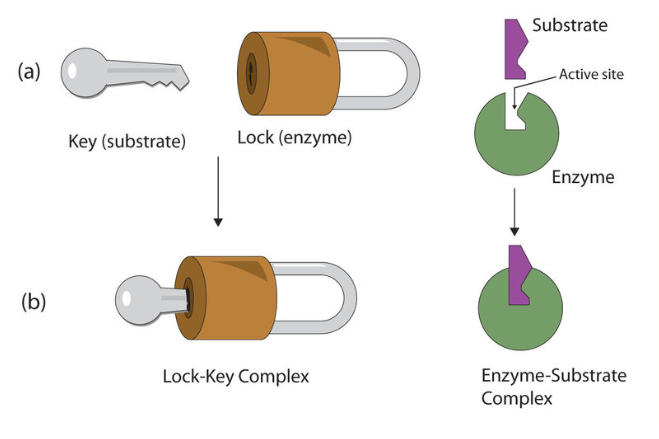
\includegraphics[width=.8\textwidth]{img/key_lock_principle.png}\\
    \source{\autocite{poshyvailo-strubeModellingSimulationsEnzymecatalyzed2015a}}
    \label{fig:LockKeyPrinciple}
    \end{minipage}
\end{figure}

The precise arrangement of amino acids in the active site allows enzymes to be highly specific for their substrates, facilitating efficient catalysis. This specificity is a key feature that enables enzymes to perform their roles in various biochemical pathways with high precision. Understanding the structure-function relationship of enzymes is essential for predicting their activities.

The prediction of pesticide degradation and the identification of enzymatic functions involved is a critical area of research with significant implications for environmental sustainability and agricultural practices. Pesticides, used globally to protect crops, often persist in the environment, leading to potential ecological and health risks. Enzymes, as biological catalysts, play a pivotal role in degrading these toxic compounds into less harmful substances. The enzymatic degradation process involves various mechanisms, predominantly microbial enzymatic activities, which catalyze reactions that transform pesticides.

For instance, reductive enzymes catalyze the reduction of pesticides, often by donating electrons and hydrogen atoms to the molecules, breaking down complex structures into simpler forms. Reductive dehalogenases, found in microorganisms like Dehalococcoides, are particularly effective in breaking down halogenated organic compounds. The efficiency of microbial enzymes in degrading soil-contaminated pesticides has been well-documented. Singh and Walker (2012) \autocite{singhMicrobialDegradationOrganophosphorus2006} highlighted the effectiveness of microbial degradation of organophosphorus compounds, while Chia et al. (2013) \autocite{chiaFunctionMicrobialEnzymes2024} discussed advancements in microbial enzymes for enhancing biodegradation processes.

Understanding these enzymatic mechanisms is crucial for predicting the enzyme classes responsible for pesticide degradation. By analyzing enzyme-pesticide interactions, it is possible to identify specific enzyme classes involved in the degradation processes. This knowledge can inform the development of more accurate predictive models for pesticide degradation, facilitating better risk assessments and environmental management strategies. Advanced computational methods, such as Deep Learning, can further enhance these predictive models by accurately identifying and classifying enzymes based on their interaction with pesticides, leading to more efficient and targeted development of new products.

\subsection{Fundamentals of Ligand Binding Site Prediction}
\label{sec:Fundamentals of Ligand Binding Site Prediction}

Enzymes interact with substrates at specific binding sites, where the catalytic reactions occur. Predicting these ligand-binding sites is crucial for understanding enzyme function. Several computational methods have been developed to predict ligand-binding sites from protein structures, including geometric, physicochemical, and machine learning-based approaches.

One approach is P2Rank, a machine learning-based tool designed for the rapid and accurate prediction of ligand-binding sites from protein structures. P2Rank uses a combination of geometric and physicochemical descriptors to analyze protein structures and predict the locations of potential binding sites. For instance, Connolly Points are regularly spaced points generated on the protein’s surface to represent solvent-accessible areas, which P2Rank analyzes to predict binding sites. These points are associated with Connolly Feature Vectors (CFVs) that describe the physicochemical properties of the protein surface.
\begin{figure}[hbt]
    \centering
    \begin{minipage}[t]{\textwidth}
    \caption{Protein (1FBL) is covered in a layer of points lying on a Connolly surface.}
    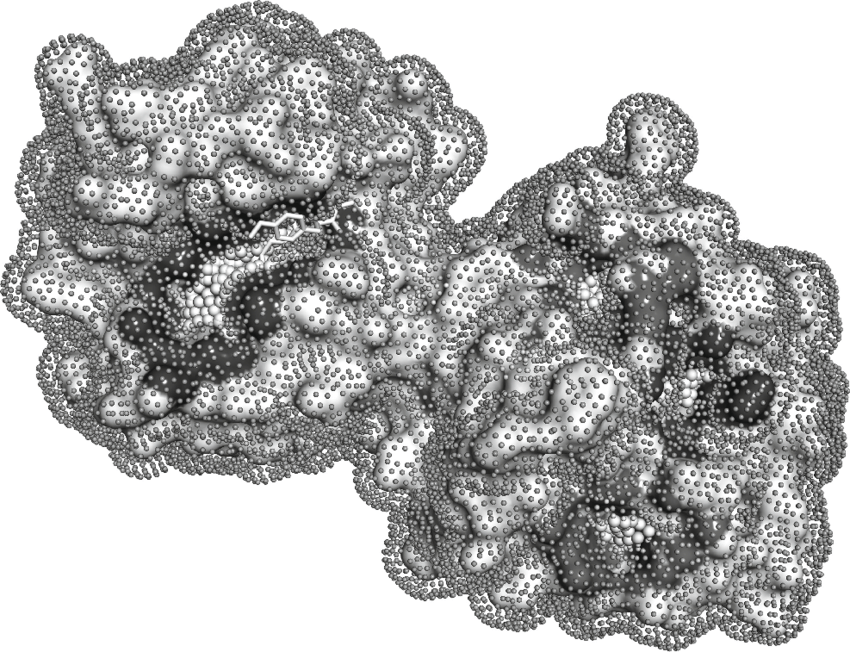
\includegraphics[width=.7\textwidth]{img/connolly-points.png}\\
    \source{\autocite{krivakP2RankMachineLearning2018}}
    \label{fig:connolly-points-p2rank}
    \end{minipage}
\end{figure}

The tool focuses on the interactive parts of enzymes, particularly the ligand-binding sites and the specific amino acids involved. This detailed analysis allows for accurate predictions of enzyme classes and their associated degradation pathways. P2Rank's ability to quickly and accurately predict binding sites makes it a valuable tool for drug discovery and environmental bioremediation applications.

P2Rank leverages local chemical neighborhood features near the protein surface to infer potential binding sites for ligands. The key steps in the P2Rank prediction process are as follows:

\begin{enumerate} 
    \item \textbf{Generation of Connolly Points}: Connolly Points are regularly spaced points generated on the protein’s Connolly surface, representing the solvent-accessible surface area of the protein. These points are generated using a numerical algorithm that ensures even spacing, typically with a solvent radius of 1.6 Å.
    \item \textbf{Calculation of Feature Descriptors}: Atomic Feature Vectors (AFVs) are calculated for each solvent-exposed heavy atom in the protein, describing various physico-chemical properties such as hydrophobicity, aromaticity, and more. These properties are projected onto the Connolly points using a distance-weighted approach, creating Connolly Feature Vectors (CFVs) for each point. The image shows Connolly Points (green dots) on the protein’s surface, where each point is associated with a Connolly Feature Vector (CFV).
    \begin{enumerate}
        \item Atomic Features: Features are inherited from the amino acid, including properties like hydrophobicity and polarity index. Additional features for AA atoms include H-Donor, H-Acceptor, and aromaticity.
        \item Aggregation of Feature Vectors: The CFV for each Connolly point is calculated by aggregating the AFVs of neighboring atoms using a distance-based weight function $w(d) = 1 - d / 6$.
    \end{enumerate}
    \item \textbf{Ligandability Prediction}: A Random Forest classifier is used to predict the ligandability score for each Connolly point, indicating the likelihood that a point is part of a ligand-binding site.
    \item \textbf{Clustering}: Connolly points with high ligandability scores are clustered using a single-linkage clustering method, representing potential binding pockets on the protein surface.
    \item \textbf{Ranking}: Each predicted pocket is assigned a score based on the cumulative ligandability scores of its constituent points, helping prioritize the most likely binding sites for further analysis or docking studies.
\end{enumerate}

P2Rank's approach can significantly enhance the accuracy of predicting enzyme-mediated degradation of pesticides by providing detailed insights into the binding interactions at the molecular level. This integration of Deep Learning and enzyme analysis forms a robust framework for developing bioremediation strategies and understanding the environmental fate of various pollutants. \autocite{krivakP2RankMachineLearning2018}

The following image illustrates an example of the P2Rank prediction for a protein structure (2SRC) with predicted ligand-binding sites:

\begin{figure}[hbt]
    \centering
    \begin{minipage}[t]{\textwidth}
    \caption{P2Rank example for 2SRC (TYROSINE-PROTEIN KINASE)}
    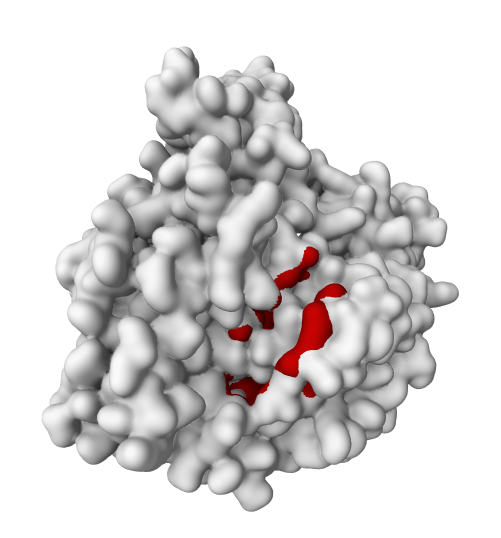
\includegraphics[width=.5\textwidth]{img/p2rank-example.png}\\
    \source{\autocite{krivakP2RankMachineLearning2018}}
    \label{fig:p2rank-example}
    \end{minipage}
\end{figure}

The red section in the image represents the predicted ligand-binding site on the protein structure, highlighting the potential interaction regions for ligands. These predicted sites can provide valuable insights into the enzyme's function and catalytic activity, aiding in the prediction of enzyme classes. By focusing on the ligand-binding pockets, P2Rank can identify the specific residues involved in the catalytic processes, enhancing the accuracy of enzyme class predictions. This specificity allows for a more nuanced analysis compared to traditional methods that utilize the entire protein sequence. By concentrating on these critical interaction sites, which are crucial for protein functions, P2Rank can identify the specific residues that are directly involved in the catalytic processes. This specificity could not only improve the accuracy of predictions but also reduce the computational complexity by focusing on smaller, more relevant regions of the protein.

\subsection{Deep Learning in Enzymology}
\label{sec:Deep Learning in Enzymology}

Deep Learning is a subset of machine learning and artificial intelligence (AI) that focuses on using neural networks with many layers (hence “deep”) to model and understand complex patterns and representations in data. Unlike traditional machine learning models, Deep Learning algorithms can automatically learn and extract features from raw input data, making them particularly powerful for tasks involving large and complex datasets, such as image recognition, natural language processing, and speech recognition. The key strength of Deep Learning lies in its ability to improve performance with more data and compute power, enabling the development of models that can achieve state-of-the-art results in various domains. \autocite{sarkerDeepLearningComprehensive2021}

Deep Learning has become an essential tool in environmental science, enabling advanced prediction and understanding of complex biochemical processes. Various Deep Learning architectures, such as the protein-transformer ESM model, have significantly impacted the prediction of biological properties from sequence data. These models can analyze vast quantities of biochemical data to predict enzyme interactions and functions, providing valuable insights into pesticide degradation mechanisms. \autocite{rivesBiologicalStructureFunction2021}

In the context of pesticide degradation and enzyme classification, such models can analyze large quantities of available biochemical data to make predictions about enzyme interactions and functions. Several Deep Learning architectures have been applied in enzyme classification and prediction tasks, from which valuable insights into the mechanism of pesticide degradation can be obtained.

For instance, the DEEPre model applies Deep Learning to predict EC numbers based on raw sequence data. Such models apply convolutional and sequential feature extraction techniques, leading to significant improvements in prediction accuracy over methods in current use. In this respect, such models may play a key role in predicting the pesticide biodegradation pathways and help to make environmental risk assessment more precise and fast. \autocite{liDEEPreSequencebasedEnzyme2017}

Despite the advances made by these models, there is still a need for new approaches to further improve the accuracy of sequence based predictions. Traditional models often rely on pre-defined features and limited datasets, which can restrict their performance and generalizability. In addition to this, many methods only focus on the prediction to the 3rd level of the EC classification, which may not provide sufficient detail for predicting pesticide degradations. For example the accuracy of EnzymeNet, a residual neural network model, across all the 4th level is 0.398. Therefore, there is a need for more advanced Deep Learning models that can predict enzyme classes with higher accuracy and resolution, enabling more precise predictions of pesticide degradation pathways. \autocite{watanabeEnzymeNetResidualNeural2023}

Current state-of-the-art models, such as DEEPre or EnzymeNet, have shown promising results in predicting enzyme classes based on sequence data. However, these models are limited in their ability to predict enzyme classes with high specificity and resolution, particularly at the 4th level of the EC hierarchy. The complexity and diversity of enzyme functions at this level pose challenges for accurate prediction, necessitating more advanced Deep Learning models. By leveraging the latest Deep Learning techniques and incorporating detailed biochemical features, it is possible to develop more accurate and efficient models for predicting enzyme classes involved in pesticide degradation.

By contrast, the proposed approach leverages the Deep Learning tool P2RANK to analyze the interactive parts of enzymes, focusing on the ligand-binding sites and the specific amino acids involved. This method can potentially provide a more detailed and accurate prediction of enzyme classes responsible for pesticide degradation, enhancing the understanding of the biodegradation pathways and mechanisms involved. Furthermore, the emphasis on ligand-binding pockets allows for a more nuanced analysis compared to traditional methods that utilize the entire protein sequence. By concentrating on these critical interaction sites, which are crucial for protein functions, P2Rank can identify the specific residues that are directly involved in the catalytic processes. This specificity could not only improves the accuracy of predictions but also reduce the computational complexity by focusing on smaller, more relevant regions of the protein. \autocite{krivakP2RankMachineLearning2018}

\subsection{Enzyme Classification with Recurrent Neural Networks}
\label{sec:Enzyme Classification with Recurrent Neural Networks}

Recurrent Neural Networks (RNNs) are a class of Deep Learning networks designed to recognize patterns in sequences of data such as text, genomes, handwriting, and spoken words. Unlike traditional feedforward neural networks, RNNs have connections that form directed cycles, allowing information to persist. This makes them particularly powerful for tasks involving sequential data, where the order of the data points matters. RNNs are designed to process sequences of data by maintaining a memory of previous inputs. This memory allows RNNs to make use of information from earlier in the sequence to influence the current processing step, which is essential for understanding context in sequential data. The fundamental difference between RNNs and traditional neural networks is the presence of loops in the network that enable the persistence of information across time steps. \autocite{schmidtRecurrentNeuralNetworks2019}

The basic structure of an RNN includes an input layer, a hidden layer with recurrent connections, and an output layer. At each time step, the hidden layer receives the input data and its own previous state, allowing it to retain and process information from previous steps in the sequence.

One of the key advancements in RNNs is the development of Long Short-Term Memory (LSTM) networks and Gated Recurrent Units (GRUs), which are designed to overcome the limitations of traditional RNNs, such as the vanishing gradient problem. These architectures use gating mechanisms to control the flow of information, making it easier to capture long-term dependencies in data.

In the context of bioinformatics, RNNs, particularly LSTMs and GRUs, are extensively used for sequence analysis tasks such as protein secondary structure prediction, gene expression analysis, and more. They are effective because they can handle the sequential nature of biological data and capture dependencies that span over long sequences. LSTM networks are a type of RNN that can learn long-term dependencies. They incorporate memory cells that can maintain their state over long periods. LSTMs have three main gates (input gate, forget gate, and output gate) that regulate the flow of information into and out of the memory cell, thus enabling the network to remember important information for longer durations. \autocite{hochreiterLongShortTermMemory1997}

The following image illustrates the basic structure of an RNN:

\begin{figure}[!htbp]
    \centering
    \begin{minipage}[t]{\textwidth}
    \caption{A diagram for a one-unit RNN.}
    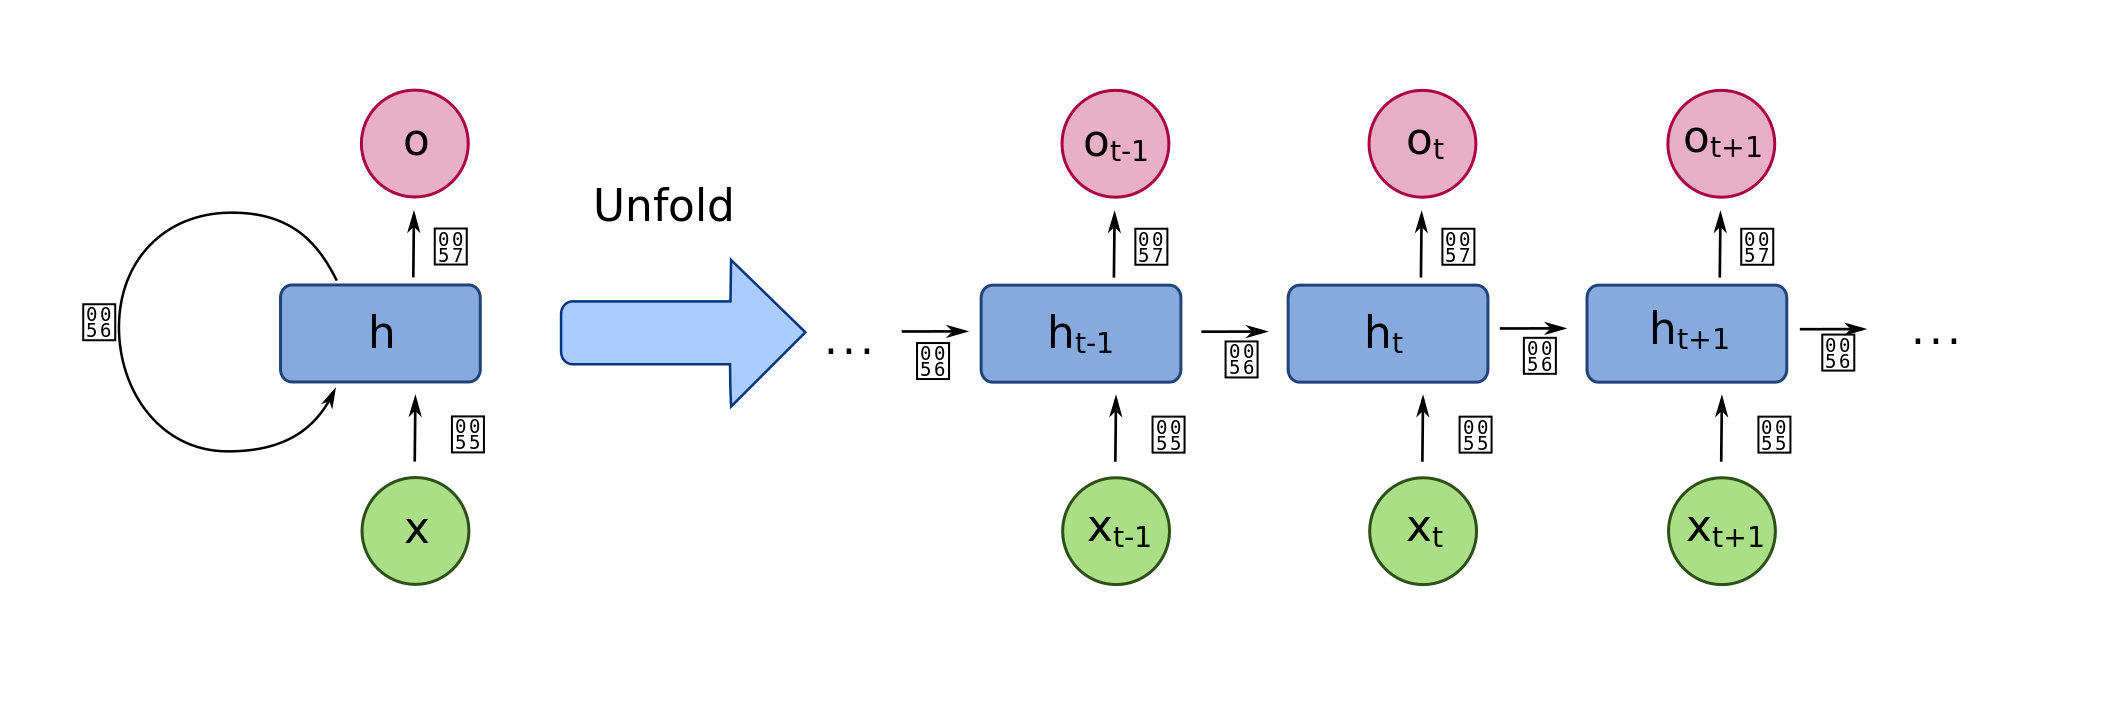
\includegraphics[width=1\textwidth]{img/Recurrent Neural Network Unfold.png}\\
    \source{\autocite{toraClassificationPuckPossession2017}}
    \label{fig:recurrent-neural-network}
    \end{minipage}
\end{figure}

\begin{enumerate}
    \item \textbf{Input Sequence (x):} In the diagram, the blue circles ($x_0, x_1, x_2, \dots, x_t$) represent the input data at different time steps. Each $x_i$ is an input vector that the network receives at a specific time step $t$. These inputs can be any sequential data, such as words in a sentence or data points in a time series.
    \item \textbf{Hidden State (h):} The purple circles ($h_0, h_1, h_2, \dots, h_t$) represent the hidden state of the network. At each time step, the hidden state $h_i$ is updated based on the current input $x_i$ and the previous hidden state $h_{i-1}$. The hidden state acts as the network's memory, retaining information about previous inputs, which is crucial for understanding sequences and making predictions based on past data.
    \item \textbf{Processing Unit (A):} The green rectangles (A) denote the recurrent unit, which processes the inputs and updates the hidden state. Each unit takes the input $x_i$ and the previous hidden state $h_{i-1}$ to produce the current hidden state $h_i$. This recurrence allows the network to maintain a chain of dependencies across time steps, enabling it to capture temporal patterns in the data.
\end{enumerate}

The recurrent connection (arrow looping back) in the hidden state allows information to persist across time steps, enabling the network to maintain context and capture dependencies in the sequence data.

In this study, RNNs are employed for predicting the enzyme class based on the amino acid sequences of a ligand binding site. The sequential nature of the amino acid sequences makes RNNs well-suited for this task, as they can capture the dependencies and patterns in the data that are crucial for predicting enzyme classes accurately. Especially for complex and long sequences, RNNs, particularly LSTMs, are effective in learning the underlying structure and relationships in the data.

\subsection{Evaluation of Deep Learning Models}
\label{sec:Evaluation of Deep Learning Models}

When developing a Deep Learning model, it is crucial to compare its performance with other models and make necessary adjustments. This process ensures that the selected model is not only the best fit for the current dataset but also generalizes well to new data. By evaluating multiple models, it is possible to identify which model architecture and hyperparameters yield the best performance. This can be done through adjusting hyperparameters such as learning rate, batch size, and network depth to optimize model performance. Techniques like dropout, L2 regularization, and batch normalization can also be used to prevent overfitting and improve model generalizability. To access the generalizability of the model, it is essential to evaluate its performance on unseen data, typically through a validation set.

To get the optimal hyperparameters, a Hyperparameter tuning is necessary. This is a critical aspect of developing Deep Learning models, as it involves selecting the optimal set of hyperparameters that maximizes the model's performance. This process can significantly impact the effectiveness of the model, as hyperparameters control various aspects of the learning process, such as the learning rate, batch size, number of epochs, and network architecture. Hyperparameters differ from model parameters as they are set before the training process begins and remain constant during training. Properly tuning these hyperparameters is essential for: \autocite{hutterAutomatedMachineLearning2019}

\begin{itemize}
    \item Optimizing the model's accuracy.
    \item Preventing overfitting or underfitting.
    \item Ensuring efficient use of computational resources.
\end{itemize}

The KerasClassifier wrapper from the keras library is used to integrate a Keras Deep Learning model with Scikit-learn's Grid Search functionality. This integration allows for systematic and efficient exploration of hyperparameter values. Grid Search involves specifying a grid of hyperparameter values and systematically evaluating the model performance for each combination. The GridSearchCV function from Scikit-learn is used to perform this exhaustive search over the specified hyperparameter space. The key hyperparameters tuned in this study include:

\begin{itemize}
    \item Optimizer: Algorithms for updating model weights (ADAM in this case).
    \item Initialization: Methods for initializing model weights (e.g., glorot uniform, normal).
    \item Epochs: Number of complete passes through the training dataset.
    \item Batch Size: Number of samples processed before the model is updated.
\end{itemize}

The Random-Grid-Search is then executed to find the best combination of hyperparameters that results in the highest model accuracy. A study by Bergstra and Bengio (2012) showed that Random Search is more efficient than Grid Search for hyperparameter optimization, as it explores the hyperparameter space more effectively. Random Search randomly samples hyperparameter values from predefined ranges, allowing for a more comprehensive search and better performance. \autocite{bergstraRandomSearchHyperParameter}

The accuracy of the model is continuously evaluated using various metrics, including precision, recall, F1 score, and accuracy. The best performance metrics are used to select the optimal hyperparameters for the model. The model is then trained using the selected hyperparameters and evaluated on the test set to assess its generalization performance. This process ensures that the model is robust and can accurately predict enzyme classes.

To effectively evaluate and compare models, various metrics are used: \autocite{sudhamathyBayesianCNNLSTMClassification2023}

\textbf{Accuracy:} Accuracy measures the proportion of correctly predicted instances out of the total instances. It is a straightforward metric but may not be reliable for imbalanced datasets.
\begin{equation}
    Accuracy = \frac{\text{Total Number of Predictions}}{\text{Number of Correct Predictions}}
\end{equation}

\textbf{Precision:} Precision indicates the accuracy of positive predictions, reflecting how many predicted positive instances are actually positive.
\begin{equation}
    Precision = \frac{\text{True Positives}}{\text{True Positives} + \text{False Positives}}
\end{equation}

\textbf{Recall:} Recall measures the model’s ability to identify all relevant instances, showing the proportion of actual positives correctly identified.
\begin{equation}
    Recall = \frac{\text{True Positives}}{\text{True Positives} + \text{False Negatives}}
\end{equation}

\textbf{F1 Score:} The F1 Score is the harmonic mean of precision and recall, providing a balanced measure when there is an uneven class distribution.
\begin{equation}
    F_1 = 2 \times \frac{\text{Precision} \times \text{Recall}}{\text{Precision} + \text{Recall}}
\end{equation}